\section{The Duffing oscillator}

\subsection{Analytical Ansatz}
As we have seen, Josephson junctions act as nonlinear inductors, hence adding nonlinearity, or anharmonicity, to an electrical circuit.
When the circuit is driven with low enough input power, the nonlinearity can be neglected.
In this case, the circuit can be described well by a driven harmonic oscillator,
\begin{align}
\ddot{x} + \delta \dot{x} + \alpha x = \gamma \cos(\omega t),
\end{align}
with the time-dependent displacement  $x=x(t)$, stiffness $\alpha$, damping $\delta$, drive amplitude $\gamma$ and drive frequency $\omega$.
All variables are assumed to be positive and real.
However, for most cases it is important to account for the anharmonicity.
The generalized mathematical model which describes such a circuit is the Duffing equation with the following equation of motion (EOM)\cite{hamelGeorgDuffingIngenieur1921}:
\begin{align}
\ddot{x} + \delta \dot{x} + \alpha x + \beta x^3 = \gamma \cos(\omega t),
\end{align}
with the anharmonicity $\beta$.

In fact, there exists an algebraic equation describing the amplitude response\cite{jordanNonlinearOrdinaryDifferential2007}:
\begin{align}
\left[ \left( \omega^2-\alpha-\frac{3}{4}\beta x^2 \right)^2 + \left( \delta\omega \right)^2 \right] x^2 = \gamma^2
\label{eq:Duffing-analytical}
\end{align}
We plot the solutions to a set of parameters ($\alpha=\gamma=1,\delta=0.1$) in Fig.\ref{fig:duffing}.

\begin{figure}
	\centering
	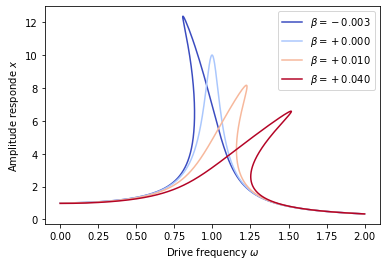
\includegraphics[width=0.7\linewidth]{chapter-theory/figs-general/duffing}
	\caption{Frequency response of Duffing oscillators for various nonlinearities and $\alpha=\gamma=1,\delta=0.1$, calculated from Eq.\ref{eq:Duffing-analytical}}
	\label{fig:duffing}
\end{figure}

\subsection{Intuitive Ansatz}
We can also take a more intuitive Ansatz to the above problem from which we can already gain qualitative information.
Let us assume the Duffing equation describes a mass on a (nonlinear) spring driven by a periodic external force.
Compared to the linear case with $F_r=kx$, the new restoring force is now given by 
\begin{align}
F_r = k^\prime x = (\alpha +\beta x^2)x.
\end{align}
For $\beta>0$, the spring is stiffened, for $\beta<0$ the spring is softened.
Quantitatively, the sign of $\beta$ does not have any effect on the behaviour of the circuit for frequency shifts small compared to the resonance frequency of the circuit.
Following first order perturbation theory, let us assume 
\begin{align}
x=x_0 \cos(\omega t)% + x_1\cos(3\omega t) + \dots
\end{align}
to be the solution of the unperturbed EOM.
If we insert this into the equation for the restoring force, we need to first calculate
\begin{align}
x^2(t) = x_0^2\cos^2(\omega t) = x_0^2\frac{1}{2}(1+2\cos(2\omega t))
\end{align}
Compared to $\cos(\omega t)$, the time average of $\cos(2\omega t)$ is zero.
Thus, the restoring force is given by
\begin{align}
F_r=k^\prime x \approx \left(k+\frac{\beta x_0^2}{2}\right)x
\end{align}
and the corresponding resonance frequency
\begin{align}
\omega \approx \omega_0 + \diff{\omega}{k}\Delta k \approx \omega_0 + \frac{\omega_0}{2}\frac{\Delta k}{k} = \omega_0 \left(1+\frac{\beta x_0^2}{4k}\right).
\end{align}
We see that the resonance frequency of the unperturbed system experiences a shift proportional to $\beta$ and the square of the position, $x_0^2$.

%\bibliography{dissertation}